%%%%%%%%%%%%%%%%%%%%%%%%%%%%%%%%%%%%%%%%%%%%%%%%%%%%%%%%%%%%%%%%%%%%%%%%%%%%%
%%%%%%%%%%%%%%%%%%%%%%%%%%%%%%%%%%%%%%%%%%%%%%%%%%%%%%%%%%%%%%%%%%%%%%%%%%%%%
\chapter{INTRODUCTION}

The aim of this thesis is to explain and apply Hidden Markov Model (HMM) and
Kalman Filter (KF) methods in context of time series prediction
problem. Istanbul Stock Exchange (ISE) and Dow Jones Industrial (DJI) index
historical prices were used as a testbed for both models and algorithms. In
order to show the capability of HMM, KF and KMM methods, various other
non-statistical methods were also used on the same dataset among which are ANNs,
polynomial fitting, and finally a simple random number generator based
predictor.

We also combined HMM, KF and KMM methods in a hybrid mechanism called KMM. This
method tries to merge both HMM, KF and KMM results through predefined weights. It was
hoped that the total would be better than the sum of its parts, that is, HMM and
KF combined could yield better and different results than each method taken
seperately. 

ISE and DJI data sets consisted of daily closing prices for over 21 years for
ISE and 30 years for DJI. DJI data was obtained from
\PVerb!http://finance.yahoo.com! site. ISE-100 historical data is available from
Turkish Central Bank site at \PVerb!http://evds.tcmb.gov.tr!. We attempted to
predict future price for 1, 5, and 10 days for each method mentioned above. All
methods were given a limited ``time window'' on which training took place, after
which, prediction for future prices could be performed. We kept the training
window the same size for all algorithms with the exception of ANN because too
much data was causing overfitting and effecting results negatively.

A natural benchmark for success of HMM, KF, KMM algorithms, or any predictive
algorithm, should be it's relative success against a random predictor. This idea
was inspired by Fama \cite{famar} where he states ``if [an] analyst can make
meaningful judgments concerning the purchase and sale of individual securities,
his choices should consistently outperform {\em randomly} selected securities of
the same general riskiness''. One can also say the worst-case performance, lower
bound of any financial predictive algorithm should be random prediction. Any
algorithm which can beat random prediction can claim that it is calculating
``some'' trend in the market that ``pure chance'' does not.

Before further delving into the details of each algorithm, we will briefly
introduce time series analysis in general, and financial time series analysis in
particular. We will provide a motivation for the methods we used, the details of
HMM, KF and KMM methods, the results of all algorithms mentioned and finally an
analysis of the outcome.

%%%%%%%%%%%%%%%%%%%%%%%%%%%%%%%%%%%%%%%%%%%%%%%%%%%%%%%%%%%%%%%%%%%%%%%%
\section{Time Series}

Time series data analysis is a natural by-product in many fields as diverse as
seismology, biology, physics, speech processing, medicine and more. Such fields
produce experimental data that needs to be analyzed using specific time series
methods and in certain cases, this analysis needs to be conducted through
probabilistic, statistical models.

Historically time series analysis was divided into two schools: {\em Frequency
  domain} and {\em time domain} approaches. Time domain approaches stated
current data was a function of earlier data and concocted an autocorrelation
function $\rho_l$ of the data, frequency approaches used spectral analysis where
Fourier transform of the autocorrelation function became important
\cite{tsay}. The sharp divisions that seemed to exist between the two approaches
seem to be settled, and at the same time the use of state space models and
Kalman filtering in 1980s caused an explosion of interest in related models for
time series analysis.

Statistical models try to explain sample data using a collection of random
variables that are in order, that fluctuate over time. For example say a time
series sample is represented by a collection of 10 random variables
$x_1,..,x_{10}$ where random variable $x_1$ represents the value of the series
at the first time point, $x_2$ at the second time point, so on. A collection of
random variables ${x_t}$ indexed by $t$ is also referred to as a stochastic
process \cite{shumway}. An excellent review of time series analysis methods can
be found in \cite{tsay}.

%%%%%%%%%%%%%%%%%%%%%%%%%%%%%%%%%%%%%%%%%%%%%%%%%%%%%%%%%%%%%%%%%%%%%%%%
\section{Financial Time Series}

Financial time series data brings forth certain issues with it from a
statistical analysis standpoint, most important of which is the interdependency
of one data point with previous data points. As a result of this
interdependency, the modeler of the data is unable to assume each point to be
independent and identically distributed (i.i.d.) which complicates the modeling
process.

The collapse of Long-Term Capital Management in 1998 proved to modelers of
financial time series that one could not see fluctuations of stock prices as
though coming from i.i.d. normal density functions. The said company based its
investment on such an model, and when it collapsed the situation threatened to
open a trillion-dollar hole in the banking industry. Since Bachelier
\cite{bachelier}, constructing finance models on Brownian Motion had been
popular until scientists started to poke holes in the theory and real-life
catastrophes such as the one above proved otherwise. Brownian Motion based
modeling requires that at each time step the price difference was a result of an
indepedent normal distribution. Fama \cite{fama} offered a detailed explanation
of the problem with that approach:

\begin{quote}
``If the population of price changes is strictly normal, on the average for any
stock ... an observation more than five standard deviations from the mean
should be observed about once every 7,000 years. In fact such observations
seem to occur about once every three to four years.''
\end{quote}

In other words Fama's findings indicated that independence assumption was
incorrect. HMM and KF methods construct a Bayesian graphical model that tries to
address this problem.

\begin{figure}[ht]
\center{
  \scalebox{0.30}{
  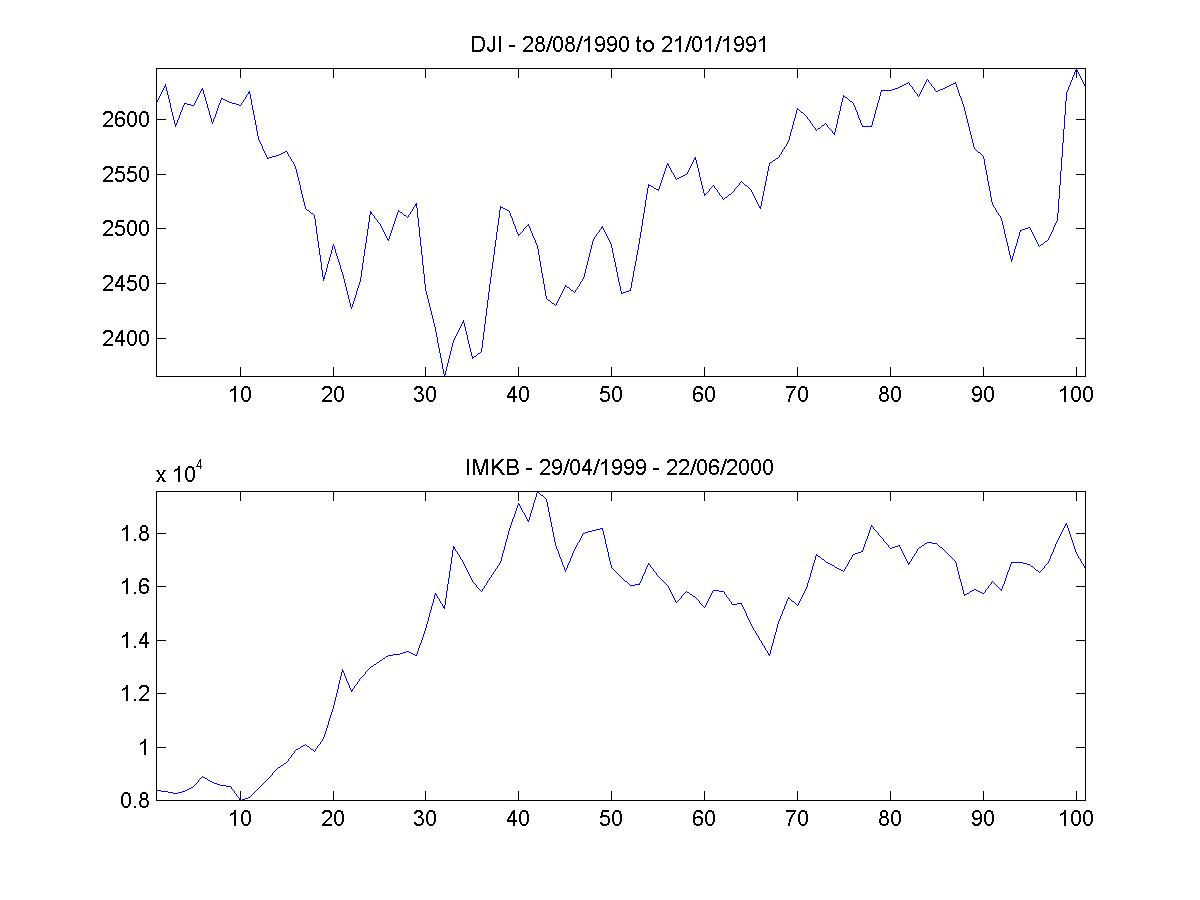
\includegraphics{./intro/somevals.jpg}
  }
}
\caption{Some Values from DJI and ISE-100}
\vspace{0.6cm}
\end{figure}


\section{Return of Financial Time Series}

We wanted to limit variations in price changes to a respectable range of values,
therefore chose to utilize rate of return of ISE and DJI price changes, instead
of the absolute values themselves. For time $t$, the return $R_t$ can be
calculated as
\begin{eqnarray*}
R_t = \frac{P_t - P_{t-1}}{P_{t-1}}
\end{eqnarray*}
where $P_t$ is the price of the financial instrument at time $t$. 

In order for HMM, KF and KMM models to learn from the data, we first pre-processed it
converting regular prices into rate of returns. This way after training and
prediction, generated values from both models would automatically be daily
returns themselves. However if an application required predictions in the form
of ``absolute stock values'', one needs go from rate of returns back to absolute
values, in this case one can simply take last absolute value for known price of
that security, and start multiplying with the predicted rate of returns
values. For example, if training was performed on $P_1,...,P_T$ where $T$ is the
amount of training points, then HMM or KF would predict returns for
$R_{T+1},...,R_{T+30}$, and using the last known price point $P_T$, we would
start multiplying our generated returns and obtain $P_{T+1},...,P_{T+30}$.

\begin{figure}[!hbp]
\center{
  \scalebox{0.30}{
  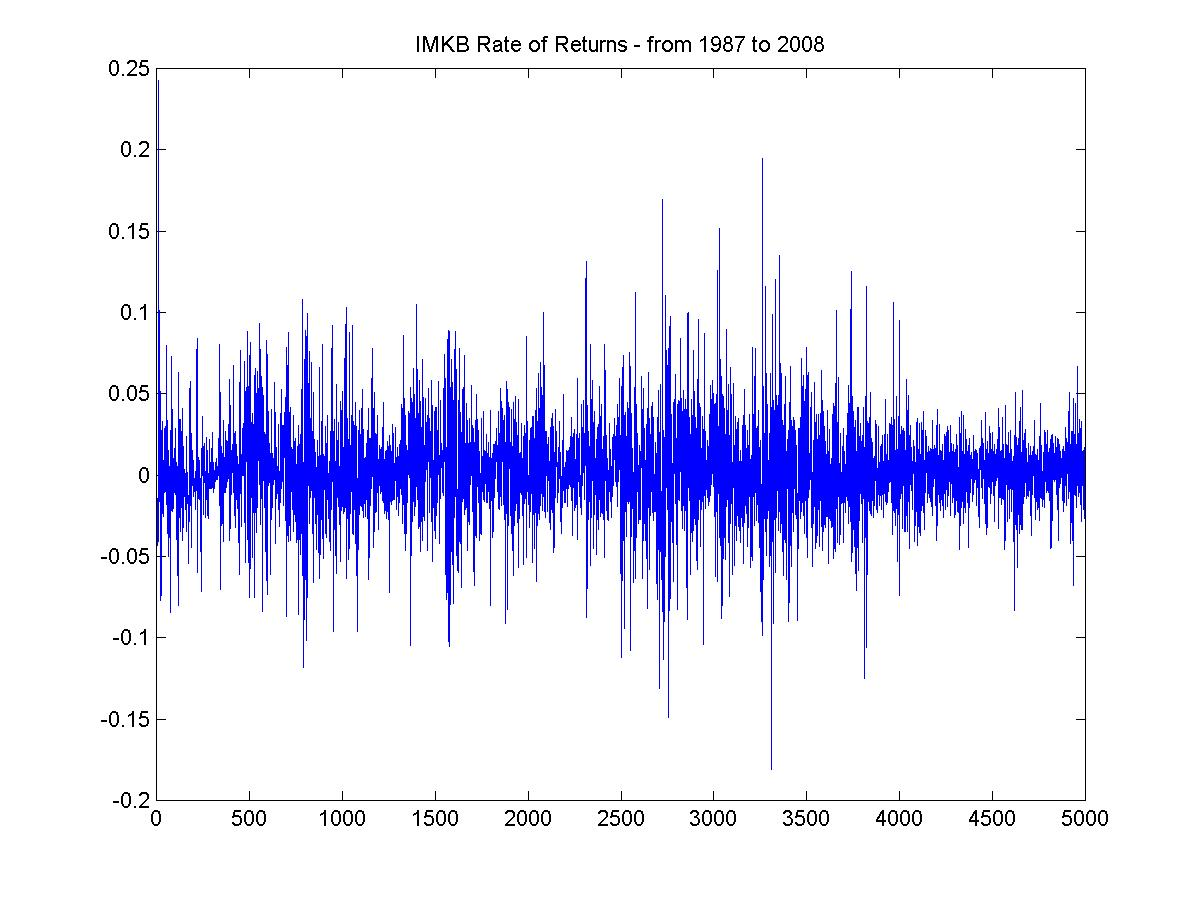
\includegraphics{./intro/volimkb.jpg}
  }
}
\caption{IMKB Volatility}
\vspace{0.6cm}
\end{figure}


%%%%%%%%%%%%%%%%%%%%%%%%%%%%%%%%%%%%%%%%%%%%%%%%%%%%%%%%%%%%%%%%%%%%%%%%
\section{Istanbul Stock Exchange and Dow Jones Industrial Data}

Now let us look at the data more closely. ISE National-100 index and Dow Jones
Industrial index are not individual stock prices themselves, instead they are
{\em summaries} over certain stock prices. This summarization capability makes
them good indicators, as economists like to say, especially an index such as
ISE-100 can signal good or bad times in the nation's stock market because of the
many number of companies' stocks it choses to reflect.

There are many methods to calculate an index. Some methods calculate a simple
average, e.g. Dow Jones Industrial index is such an average. 30 industrial
companies with high enough valuation in New York Stock Exchange were picked to
form this index, and the stock price for all 30 companies were simply averaged
to obtain a final DJI value.

ISE National-100 index on the other hand, is an index that is a weighted average
- it takes more than one parameter to calculate a final result and it assigns
different weights to each financial instrument. The formula is
\begin{eqnarray*}
E_t = \frac{\sum_{i=1}^n F_{it} N_{it} H_{it}}{B_t}
\end{eqnarray*}
where\\
$E_t$: The value of index at time $t$\\
$n$: The number of companies that contribute to the index' calculation\\
$F_{it}$: The value of $i^{th}$ stock at time $t$\\
$N_{it}$: The total number of shares outstanding of the stock $i$ at time $t$. \\
$H_{it}$: The flotation weight (publicly-held portion, i.e. the ratio of stocks
kept in custody at Takasbank, except those kept in non-fungible accounts) of the
stock $i$ at period $t$. \\
$B_t$: The value of divisor at period $t$ (Adjusted base market value). \\

Here are some statistics on the DJI and ISE data:

\vspace{0.3cm}

\begin{table}[!h]
\caption{Istanbul Stock Exchange}
\vspace{0.3cm}
\begin{tabular}{|l|l|l|l|l|l|l|l|}
\hline
Size & Mean & Var & Kurtosis & Skew & J.Bera Null & Min & Max \\
\hline
5045 & 0.00214 & 0.0008 &     6.9154 &     0.2745 &  1 & -0.1811 & 0.242 \\
\hline
\end{tabular}
\end{table}

\vspace{0.3cm}

\begin{table}[!h]
\caption{Dow Jones Industrial}
\vspace{0.3cm}
\begin{tabular}{|l|l|l|l|l|l|l|l|}
\hline
Size & Mean & Var & Kurtosis & Skew & J.Bera Null & Min & Max \\
\hline
9341 & 0.00035 & 0.0001 &    34.40 &    -1.15 &     1 &    -0.226 & 0.101 \\
\hline
\end{tabular}
\end{table}

Notable statistics presented above are kurtosis, skew and Jarque-Bera
test. Skewness is a measure of asymmetry, visually a distribution with positive
skewness would have a so-called tail much longer on its right side than on its
left. The reverse statement is true for negative skewness - such distributions
would have a longer tail on the left side of its graphic. Longer tail on one
side means more data would come from that side of that distribution.

\begin{figure}[!h]
\center{
  \scalebox{0.55}{
  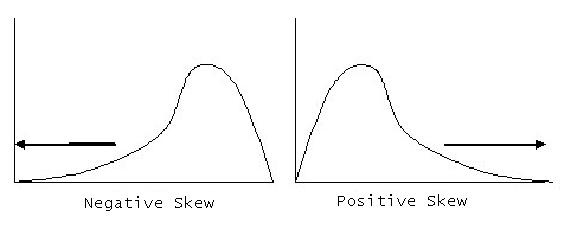
\includegraphics{./intro/skew.JPG}
  }
}
\vspace{0.6cm}
\end{figure}

Mathematically, skewness is the third standardized moment $\gamma_1$ calculated
as 
\begin{eqnarray*}
\gamma_1 = \frac{\mu_3}{\sigma^3}
\end{eqnarray*}
where $\mu_3$ is the third moment and $\sigma$ is the well-known standard
deviation. Skewness can signal us if one can assume a distribution is
Gaussian. Gaussian distribution has a skewness of zero, hence if sample skewness
of a distribution is non-zero, we can conclude that this distribution is not
Normal. 

Kurtosis, another important metric, tells us something about the presence of
extremely high values in the data. Standard normal distribution has a kurtosis
of zero, higher kurtosis values signal the presence of sharper peak in the
distribution, lower kursosis distributions tend to have flatter peaks. In other
words, kurtosis metric can tell us if extreme values are found more commonly in
a distribution or not. The formula for kurtosis is 
\begin{eqnarray*}
\frac{\sum_{i=1}T(X_i - \bar{X})^4}{(T-1)\sigma^4}
\end{eqnarray*}
Taken together skewness and kurtosis metrics can indicate if a distribution is
normal. There is also a goodness-of-fit measure called Jarque-Bera test that can
indicate normalty of a distribution. This test combines skewness and kurtosis
measures to accept or reject the null hypothesis that the distribution in
question is normal.

Looking at skewness and kurtosis for ISE and DJI data sets, we can see kurtosis
value is very high for both of the sets. This means there are a lot of extreme
values present in the sample data. It can also be observed that ISE-100 is
skewed positively, though not by much, and DJI data is skewed negatively. It is
known in finance literature that stock markets are skewed negatively because
decreases are much sharper than increases. An hypothesis as to why claims that
the reason is related to basic human psychology: At time of crises, people panic
and group mentality tempts a big number of people to sell their stocks at the
same time, hence causing sharper decreases than increases in the stock market
data. The claim seems to be justified by the presence of certain ``brakes'' in
the market in almost all markets in the world with the help of which, if daily
market decrease passes a certain predefined threshold, all activity in the
market is stopped until the next day. The goal here is giving traders time to
think and calm down, trying to offset the selling histeria that might be caused
in a moment of confusion. 

We mentioned almost all markets are skewed negatively, then we need to explain
why ISE-100 skewed positively. The reason here could be that ISE is a relatively
young market and the composition of ISE-100 index has changed over the years,
hence the sample skewness for 20 years worth of data points (as we have done)
might not offer the best results. We hypothized taking later years' data points
would offer negative skewness. This turned out to be correct, a skewness
calculation for around last 8 years did indeed offer a negative result.

%%%%%%%%%%%%%%%%%%%%%%%%%%%%%%%%%%%%%%%%%%%%%%%%%%%%%%%%%%%%%%%%%%%%%%%%
\section{Classic Methods: ARCH, GARCH, EGARCH models} 

Least squares models have been used on financial time series data for many
years. One of the important assumptions that least squares based analysis makes
is the variance of error terms stays the same throughout the time series. This
assumption, which is called homoskedasticity, does not seem to hold for
financial time series data consistently. It has been shown that the reverse
condition is true, called heteroskedasticity, that posits the variance of the
error changes. ARCH/GARCH methods attempt to model this variance \cite{engle}.

ARCH stands for \textbf{a}uto\textbf{r}egressive \textbf{c}onditional
\textbf{h}eteroskedasticity, and GARCH is \textbf{g}eneral ARCH. First proposed
by Engle \cite{engle3} then Bollershev \cite{bollershev}, these models try to
put forth a correlation between variance of error at time $t$ and variance on
days preceding $t$. The reason for such relationship is the fact that volatility
seems to have ``regions'' as observed by Mandelbrot in \cite{mandelbrot} - he
stated that in rate of return data ``large changes tend to be followed by large
changes, of either sign, and small changes tend to be followed by small
changes''. This and similar observations led to an array of research on
volatility clustering using methods such as ANN and many other statistical
tools. (G)ARCH methods are one of these methods which try to forecast volatility
based on historical rate of return data. As of 1992, a survey showed over 200
papers had used (G)ARCH and related models for financial time series
\cite{engle2}.

As shown in \cite{engle2}, let $r_t$ be the rate of return of a stock from time
$t-1$ to $t$, and $F_{t-1}$ be ``information'' that is relevant to make a
decision about buying or selling a security at time $t-1$. Then the expected
rate of return at time $t$ can be shown as $E(r_t|F_{t-1})$ and the variance can
be shown as $Var(r_t|F_{t-1})$. Let us call the former $m_t$ and the latter
$h_t$. Engle \cite{engle3} suggests that $h_t$ can be modeled as a function of
$\epsilon_t$ which is the error calculated as $\epsilon_t = r_t - m_t$. In a
ARCH(p) model this can be shown as 
\begin{eqnarray*}
h_t = \omega + \sum_{i=1}^p \alpha_i\epsilon_{t-i}^2
\end{eqnarray*}

where $\omega$, $\alpha_1,..,\alpha_p$ and $p$ are all constants which (except
$p$) are to be estimated from the past historical data. According to this
ARCH(p) model, past errors (news) older than $p$ periods have no effect on the
current day.

GARCH(p,q) model invented by Bollershev \cite{bollershev} generalizes ARCH(p)
model as
\begin{eqnarray*}
h_t = \omega + \sum_{i=1}^p \alpha_i \omega_{t-1}^2 + \sum_{i=1}^q \beta_i h_{t-i}
\end{eqnarray*}
where $\alpha_1,..,\alpha_p,\beta_1,...,\beta_p$ and $\omega$ are constants. 

EGARCH model proposed by Nelson \cite{nelson} attempts to correct problems in
(G)ARCH modeling that stem from the asymetric nature of the stock price data:
Statistical analysis of volatility showed that drops in markets are sharper and
deeper than increases as we have seen previously. In comparison good news in the
market is taken in much more rationally and causes more moderate increases than
decreases. (G)ARCH models do not take this asymetry into account which EGARCH
models attempt to correct. EGARCH is formulized as
\begin{eqnarray*}
log(h_t) = \omega + \beta \cdot log(h_{t-1}) + 
\gamma \frac{\epsilon_{t-1}}{\sqrt{h_{t-1}}} + 
\alpha \bigg[ \frac{|\epsilon_{t-1}|}{\sqrt{h_{t-1}}} - \sqrt{2 / \pi} \bigg]
\end{eqnarray*}
where $\omega,\beta,\gamma$ and $\alpha$ are constants. As a result of this
formulation positive $\epsilon$ values generate less volatility than negative
values - or good news have less effect than bad news. Mathematically, out of two
$\epsilon$ values that have the same absolute value but different signs, the
negative one would cause more increase. Notice how $\gamma$ in $\gamma \cdot
\epsilon_{t-1} / \sqrt{h_{t-1}}$ can now capture the sign of earlier $\epsilon$
values, whereas in ARCH and GARCH models this term was squared causing only the
amplitude of $\epsilon$ to contribute to the model, whether it was negative or
positive. Also, EGARCH model assures that ``bigger'' news have ``greater''
impact on volatility which GARCH model does not take into account \cite{engle2}.

All ARCH variants with preference being on GARCH and EGARCH have been found
quite successful in predicting market volatility. We did not use them in our
comparison of prediction methods. 

%%%%%%%%%%%%%%%%%%%%%%%%%%%%%%%%%%%%%%%%%%%%%%%%%%%%%%%%%%%%%%%%%%%%%%%%%%%%%
\section{Artificial Neural Networks}

ANNs are biologically inspired constructs which are used heavily in robotics,
time series analysis, signal filtration, regression and classification. ANNs are
built to mimic neurons in human brain which can receive signals through
dendrites, and emits them through axons to snyapses, then the signal is
transmitted to the next neuron in the chain.

\begin{figure}[h]
\center{
  \scalebox{0.8}{
  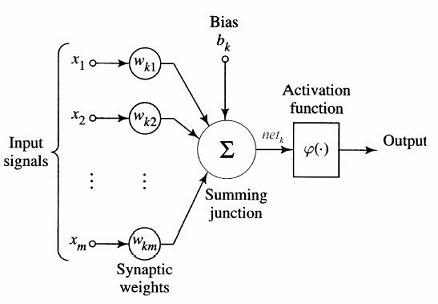
\includegraphics{./intro/neuron.JPG}
  }
}
\caption{A neuron}
\vspace{0.6cm}
\end{figure}

A network with one layer of neurons is called a perceptron. If there is more
than one layer available, this network is called a multilayer perceptron
(MLP). For the purposes of this thesis, we used an MLP for our time series
analysis tasks. It has been proven that an MLP with single hidden layer and
sufficient number of neurons can approximate any function. This is an
improvement over single layer regular perceptron which has problems with the
infamous XOR function.

ANNs are trained with using data sets whose contents include a set of input
points $x_1,..,x_N$ along with output data point(s) $y_1,..,y_K$. At each
training step, the current state (weights of the neurons) of ANN is used to
calculate an error between predicted and real output values, then, the weights
of the hidden neurons are modified in order to decrease the error value. This is
performed for all data points in the training data set. The error measure $J$ is
\begin{eqnarray*}
J = \frac{1}{2N}\sum_{i=1}^n (\hat{y}_i - y_i)^2
\end{eqnarray*}
Gradient descent with back propagation is a popular method to minimize the error
function at each iteration. 

For stock price prediction purposes, we utilized an MLP network with 30 neurons
in the hidden layer, input size 300, one output and linear activation
function. We used a Matlab\textsuperscript{\textregistered} package called
Netlab as our ANN package written by Christopher Bishop and Ian Nabney.

Time series data had to be tailored so it could be fed into a neural network. In
applications such as face recognition, flattening out the input matrix into one
continous vector $\mathbf{x}$ and mapping this flattened structure to a single
classification code is quite natural. With time series, data the mapping of
input to outputs is somewhat less intuitive. The trick is using autoregression -
having the time series contain both the input and the output at the same time
where one data input set $x_1,...,x_N$ can act as input and $x_{N+1}$ can act as
output, next input would be $x_2,...,x_{N+1}$ as input and $x_{N+2}$ as output
and by shifting by one, so on. With this method, at each iteration we
essentially are creating a new dataset which contains a set of input/output
matchings.

To make predictions, we feed ``current data'' starting from today going back as
much as input allows, as a new input collection, and the single output value is
then the prediction for tomorrow's stock price. If we need to make prediction
for more than one day, we treat each newly generated predicted value as another
input, folding it into the same time series sequence as the rest of the input
data. Naturally this would cause predictions to worsen as part of the input data
starts consisting of not actual data but predicted data, but if the modeler
keeps the projected days to a minimum, the algorithm can produce acceptable
results.

%%%%%%%%%%%%%%%%%%%%%%%%%%%%%%%%%%%%%%%%%%%%%%%%%%%%%%%%%%%%%%%%%%%%%%%%%%%%%
\section{Polynomial Regression}

Another simple yet powerful method used for comparion was a method that falls
under linear regression umbrella, called polynomial regression. With this model,
given data for $y$ and $x$ pairs, the relation between them is assumed to be

\begin{eqnarray*}
y = \beta_0 + \beta_1x + ... + \beta_1x^k + \epsilon
\end{eqnarray*}

In order to fit the model to the data, the modeler first decides the order of
the polynomial equation (we used 10). Then, a least squares fit is performed
which aims to minimize the error $\epsilon$. At the end this process outputs all
$\beta$ coeffecients to define the equation for $y$. Matlab's \PVerb!polyfit!
accomplished this task.

During modeling process, we first tried ``time'' variable as $x$ and obtained
less than satisfactory results. Next we decided to divide up the historical
stock price data in two parts, and have $i^{th}$ element of first part to be
$x$, and $i^{th}$ element of second part to be its matching $y$, then do this
for all elements of first and second parts. On this data set, we could fit the
polynomial equation to the data giving us the $\beta$ values.

\begin{figure}[h]
\center{
  \scalebox{0.55}{
  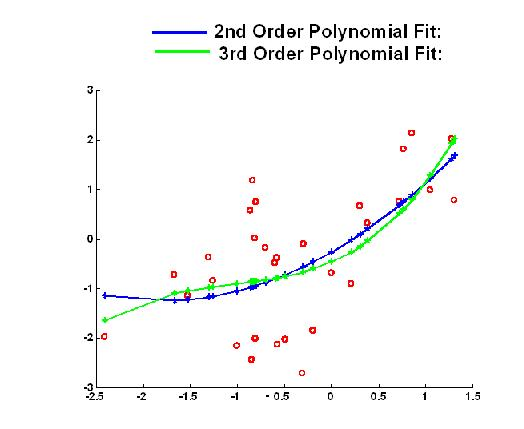
\includegraphics{./intro/poly.JPG}
  }
}
\caption{Example of Polynomial Fitting}
\vspace{0.6cm}
\end{figure}

For prediction, if we need to estimate $N$ days in the future, then we go back
$N$ days starting from today, hence the historical $N$ points became our new
$x$'s, plugging each $x$ into our ``learned'' polynomial equation would give us
future $y$'s.

%%%%%%%%%%%%%%%%%%%%%%%%%%%%%%%%%%%%%%%%%%%%%%%%%%%%%%%%%%%%%%%%%%%%%%%%%%%%%
\section{Kalman and HMM Markov Models}

In order to obtain better prediction, we hypothesized a combination of HMM and
KF methods could yield different, hopefully better results. We called this
method KMM, a combination of words \textbf{K}F and H\textbf{MM}. There are
various methods in the literature to combine more than one predictor, or
``experts'', for a certain data set. One method is assigning a different expert
for each seperate region, training it, then combining all local experts to
arrive at a better global predictor.

Another method is combining the output of each expert for each data point
prediction. This way, every expert is contributing something to the overall
result, although through different weights. Mathematically every data point
$y_i$ is a combination of
\begin{eqnarray*}
y_i = \sum_j w_j o_{ij}
\end{eqnarray*}
where $o_{ij}$ is prediction from expert $j$ at time $i$, and $w_j$ is the
weight assigned to expert $j$. The sum of weights for all experts must equal to
one, that is, $\sum_j w_j = 1$. 

\begin{figure}[h]
\center{
  \scalebox{0.55}{
  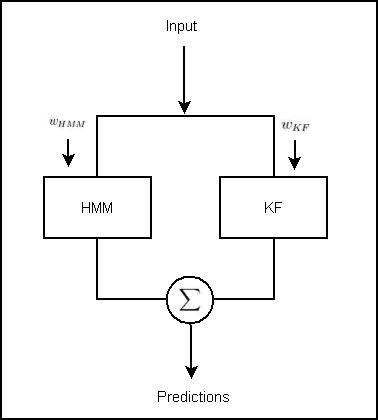
\includegraphics{./intro/kmm.jpeg}
  }
}
\caption{KMM Structure}
\vspace{0.6cm}
\end{figure}


%%%%%%%%%%%%%%%%%%%%%%%%%%%%%%%%%%%%%%%%%%%%%%%%%%%%%%%%%%%%%%%%%%%%%%%%
\section{Previous Work} \label{prevwork}

Using HMM and KF for financial time series prediction is a well known method. As
stated in \cite{ghahramani3} and confirmed by a quick look in to the literature
shows that most probabilistic time series models of use today are descendants of
either HMMs or state space models (SSMs). There is one approach that combines
both HMM and KF methods proposed by Ghahramani and Hinton. They divide the data
into multiple regions detected by HMM, then for each segment, a SSM is trained
as an ``expert'' for that region. In other words, for any given data point, SSMs
are competing among each other to describe that data point. Once SSMs are
trained, the overall flow over those ``multiple regions'' -multiple SSMs- can be
handled by the HMM. There is a similar method called Hidden Markov Experts (HME)
proposed by Shi and Weigend \cite{shi}. HME also utilizes seperation of regions
using HMMs but connects them by using ANNs \cite{nabney}.

Gürgen and Yümlü \cite{gurgen}, employed neural mixture of experts (MOE)
structure for ISE prediction and compared those results with an ANN, a
polynomial and a radial basis function (RBF) nets.

Hassan and Nath \cite{hassan} use HMMs in a way similar that is used in speech
recognition. They decided to train one HMM {\em per trading day} and used four
values of each day in sequence as a mini-time series. Those values were opening
price, high price, low price and closing price. The modeler trains one HMM per
trading day using the four values and also remembers the next day's closing
price. This will become useful for prediction, during which, four values of
yesterday are passed to every trained HMM one by one. Then, whichever HMM
reports the highest likelihood for those four mini time series points, that HMM
is picked as the correct HMM to predict tomorrow. Of course even though the
match gives a change pattern that might be similar to values from yesterday, the
absolute values of both sides can be different - in which case prediction
program simply ``adds'' the average difference of values from matched HMM to
tomorrows predicted stock price. This method \cite{hassan} predicts only one day
ahead.

